%xelatex -shell-escape -output-directory=bin ergasia.tex
\documentclass{assignment}

\usepackage{enumerate} % Για την χρησιμοποίηση roman enumerate
\usepackage{paralist} % για το περιβάλλον inparaenum που είναι οι λίστες μέσα στο κείμενο.

\title{Αναγνώριση Προτύπων \\ Θέμα Εξαμήνου }
\date{Αθήνα, 2014}

\author{Αναγνωστόπουλος Βασίλης - Θάνος (ΜΠΠΛ 13002)}

\begin{document}

\maketitle
% Να σκεφτώ τί αλλαγές θέλω να κάνω με τις αριθμήσεις και άμα θέλω να κάνω.
% Να σκεφτώ να τις ενσωματώσω και στο assignment.cls

\setcounter{page}{1} 
\pagenumbering{roman}

\pagestyle{plain}
\tableofcontents
%\listoftables
\listoffigures
%\renewcommand\listoflistingscaption{Κατάλογος πηγαίου κώδικα}
%\listoflistings
\newpage

%\pagestyle{headings}
%\pagestyle{fancy}
\setcounter{page}{1} 
\pagenumbering{arabic}

\section{Άσκηση 1η}
\subsection{Εκφώνηση}

Να γίνει πλήρης βιβλιογραφική έρευνα με βάση τις λέξεις κλειδιά "\en{Artificial Immune System}".

\subsection {Λύση}

\section{Άσκηση 2η}
\subsection{Εκφώνηση}

Να γίνει πλήρης βιβλιογραφική έρευνα με βάση τις λέξεις κλειδιά "\en{Swarm Intelligence}".

\subsection {Λύση}

\section{Άσκηση 3η}
\subsection{Εκφώνηση}

Να γίνει πλήρης βιβλιογραφική έρευνα με βάση τις λέξεις κλειδιά "\en{Evolutionary Computing}" και \en{Genetic Algorithms}.

\subsection {Λύση}

σελ. 80

\section{Άσκηση 4η}
\subsection{Εκφώνηση}

Να γίνει πλήρης βιβλιογραφική έρευνα με βάση τις λέξεις κλειδιά "\en{Fuzzy Logic Systems}".

\subsection {Λύση}

Η ασαφής λογική πρόκειται για μία γενίκευση της συμβατικής Θεωρίας Συνόλων και είναι μία πλειότιμη λογική η οποία ασχολείται με την λογική σαν μία προσέγγιση και όχι σαν κάτι σταθερό και ακριβές \cite{engelbrecht,class_notes,wiki:fuzzy_logic,zadeh1994}. %Fuzzy logic is a form of many-valued logic which deals with reasoning that is approximate rather than fixed and exact.

Η ασαφής λογική βασίζεται στα ασαφή σύνολα. Σε σύγκριση με τα δυαδικά σύνολα (οι μεταβλητές των οποίων μπορούν να λάβουν την τιμή "αλήθεια" ή "ψευδές"), τα ασαφή σύνολα περιέχουν αντικείμενα τα οποία ικανοποιούν ανακριβείς ιδιότητες και μπορεί να έχουν μία τιμή αληθείας η οποία κυμαίνεται στο βαθμό μεταξύ 0 και 1 σε αυτό το σύνολο (βλ. εξίσωση \eqref{eq:fuzzy_set}) \cite{zadeh1965338}. 

\begin{equation}
\mu_A : X \rightarrow [0,1]
\label{eq:fuzzy_set}
\end{equation}

όπου $X$ ο χώρος των αντικειμένων. Αν $x$ ένα γενικό αντικείμενο του $X$ με $x \in X$ τότε το $\mu_A(x)$ δείχνει την βεβαιότητα με την οποία το στοιχείο $x$ ανήκει στο ασαφή σύνολο $A$.

Ο βαθμός συμμετοχής σε ένα ασαφές σύνολο υποδηλώνει την βεβαιότητα (ή την αβεβαιότητα) ότι το στοιχείο ανήκει σε αυτή την ομάδα. Η ασαφής λογική χρησιμοποιείται για να χειριστεί την έννοια της μερικής αλήθειας, όπου η τιμή της αλήθειας μπορεί να κυμαίνεται μεταξύ εντελώς αλήθειας και εντελώς ψευδή. Τα ασαφή σύνολα επιτρέπουν την μοντελοποίηση των αβεβαιοτήτων της φυσικής γλώσσας και μπορούν να χρησιμοποιηθούν τόσο για διακριτούς ή/και συνεχόμενους χώρους \cite{engelbrecht,class_notes,wiki:fuzzy_logic}. 

Για τον πλήρη ορισμό ενός ασαφές συνόλου χρειαζόμαστε ακόμα και την συνάρτηση μέλος του ασαφούς συνόλου, η οποία χρησιμοποιείται για να συνδέσει τον βαθμό συμμετοχής κάθε στοιχείου $x$ του χώρου των αντικειμένων με το αντίστοιχο ασαφές σύνολο. Οι συναρτήσεις μέλη μπορεί να έχουν οποιοδήποτε σχήμα ή τύπο (βλ. σχήμα \ref{fig:fuzzy_logic_membership_function}). \cite{engelbrecht}.

\begin{figure}[htbp]
  \centering
  \begin{subfigure}[b]{0.5\textwidth}
     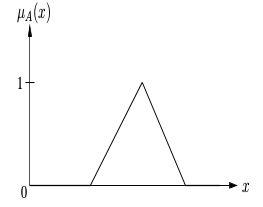
\includegraphics[width=\textwidth,height=0.25\textheight]{images/fuzzy_logic_membership_function_triangular.png}
  \caption{Τριγωνική συνάρτηση μέλους}
  \end{subfigure}%
   ~ %add desired spacing between images, e. g. ~, \quad, \qquad, \hfill etc.
  \begin{subfigure}[b]{0.5\textwidth}
    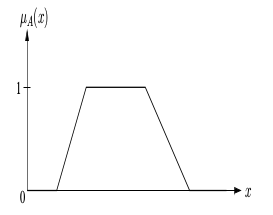
\includegraphics[width=\textwidth,height=0.25\textheight]{images/fuzzy_logic_membership_function_trapezoidal.png}
  \caption{Τραπεζοειδής συνάρτηση μέλους}
  \end{subfigure}
   ~ %add desired spacing between images, e. g. ~, \quad, \qquad, \hfill etc.
  \begin{subfigure}[b]{0.4\textwidth}
    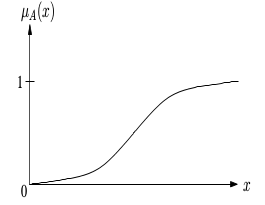
\includegraphics[width=\textwidth,height=0.25\textheight]{images/fuzzy_logic_membership_function_logistic.png}
  \caption{Λογιστική συνάρτηση μέλους}
  \end{subfigure}
   ~ %add desired spacing between images, e. g. ~, \quad, \qquad, \hfill etc.
  \begin{subfigure}[b]{0.5\textwidth}
    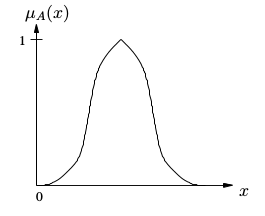
\includegraphics[width=\textwidth,height=0.25\textheight]{images/fuzzy_logic_membership_function_gaussian.png}
  \caption{Γκαουσιανή συνάρτηση μέλους}
  \end{subfigure}
  \caption{Παραδείγματα συναρτήσεων μελών \cite{engelbrecht}}
\label{fig:fuzzy_logic_membership_function}
\end{figure}

Ένα σύστημα ασαφούς λογικής (αγγλ. \en{Fuzzy Logic Systems - FLS}) είναι μία γραμμική απεικόνιση ενός διανύσματος δεδομένων εισόδου (χαρακτηριστικά) σε μία βαθμωτή έξοδο (η οποία αποσυντίθεται σε μία συλλογή από ανεξάρτητες πολλαπλές εισόδου/μονής εξόδου σύστημα) \cite{mendel364485,class_notes}.

\begin{figure}
\begin{center}
\resizebox*{\textwidth}{!}{
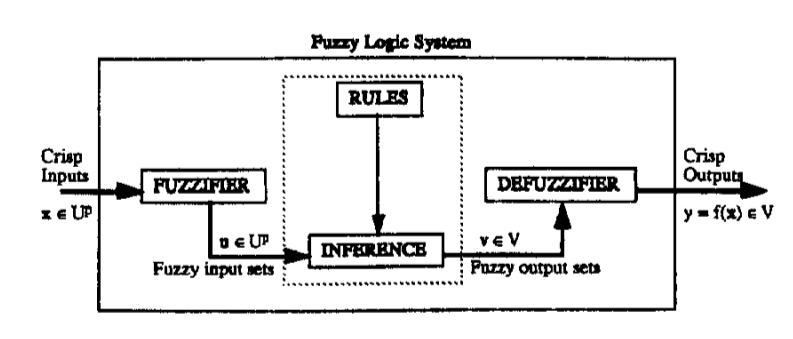
\includegraphics{images/fuzzy_logic_system.png}}
\caption{Σύστημα ασαφούς λογικής \cite{mendel364485,class_notes}}
\label{fig:fuzzy_logic_system}
\end{center}
\end{figure}


σελ. 59

\section{Άσκηση 5η}
\subsection{Εκφώνηση}

Να υλοποιηθούν αλγόριθμοι ιεραρχικής ομαδοποίησης δεδομένων και να εφαρμοστούν στα δεδομένα εκφράσεων προσώπου που θα σας παρασχεθούν.

\subsection {Λύση}


σελ. 56



\phantomsection \label{Βιβλιογραφία}
\addcontentsline{toc}{section}{Βιβλιογραφία}
%\mtcaddchapter[Βιβλιογραφία] % Λόγω του minitoc
\bibliographystyle{plain}
\bibliography{references}

\newpage

\end{document}

